\subsection{Implementierung des Anwendungsservers}

Für den Prototypen wurden das PHP-Framework \trademark{Symfony2}\footnote{\url{http://symfony.com/}} eingesetzt, das von sich aus bereits viele Anforderungen aus dem vorangegangenen Abschnitt erfüllt. Da im Kern jeder Web-Anwendung HTTP-Anfragen beantwortet werden, überträgt \trademark{Symfony2} dieses Paradigma auf die Art und Weise, wie im Framework Anfragen verarbeitet werden: mit Hilfe einer Routen-Konfiguration werden Controller für auf bestimmt Pfade in der Anfrage-URL registriert und vom Framework automatisch instanziert und aufgerufen. Die Controller schreiben dann ihre Antwort in ein Antwort-Objekt, das vom Framework als Antwort gesendet wird. Oberstes Prinzip bei der Entwicklung des Frameworks war die Modularisierung und die Wiederverwendbarkeit, so dass alle Komponenten nur mit Hilfe eines Service-Containers kommunizieren. Dadurch sind \trademark{Symfony2} besonders leicht zu warten und auch zu testen, entsprechende Unit-Testing-Komponenten werden bereits mitgeliefert.

\subsubsection{API}

Alle Funktionen des Anwendungsservers sind über eine Schnittstelle verwendbar, die JSON-Objekte enthalten dabei Zusatzinformationen zum Kontext und zu Relationen, wie in Abschnitt \ref{l:anbindung-gui} / S.\pageref{l:anbindung-gui} beschrieben. 

\begin{samepage}
\begin{verbatim}
{
    "@context":"http://jsonld.retext.it/Container",
    "@subject":"/api/container/4fdf26e7820b905118000001",
    "@relations":[
        {
            "@context":"http://coderbyheart.de/jsonld/Relation",
            "relatedcontext":"http://jsonld.retext.it/Project",
            "href":"/api/project/4fdf26e7820b905118000000",
            "list":false
        },
        {
            "@context":"http://coderbyheart.de/jsonld/Relation",
            "relatedcontext":"http://jsonld.retext.it/Element",
            "role":"http://jsonld.retext.it/ontology/child",
            "href":"/api/element?parent=4fdf26e7820b905118000001",
            "list":true
        },
        …
    ],
    "id": "4fdf26e7820b905118000001",
    "name": "Abschnitt 1",
    …
}
\end{verbatim}

Dieses Listing zeigt als Beispiel das JSON-Objekt eines Containers. In der \texttt{@relations}-Liste ist der Verweis auf das Eltern-Element enthalten, aber auch auf die Liste mit untergeordneten Elementen dieses Containers. Im Client werden die Relationen je nach Bedarf durchsucht und die passende ausgewählt, sofern weitere Daten benötigt werden. Die jeweilige URL ist in \texttt{href} enthalten, so dass sich im Quellcode des Clients nur wenige hart-kodierte Endpunkte finden.

\end{samepage}

\subsubsection{Persistenz}

\begin{center}
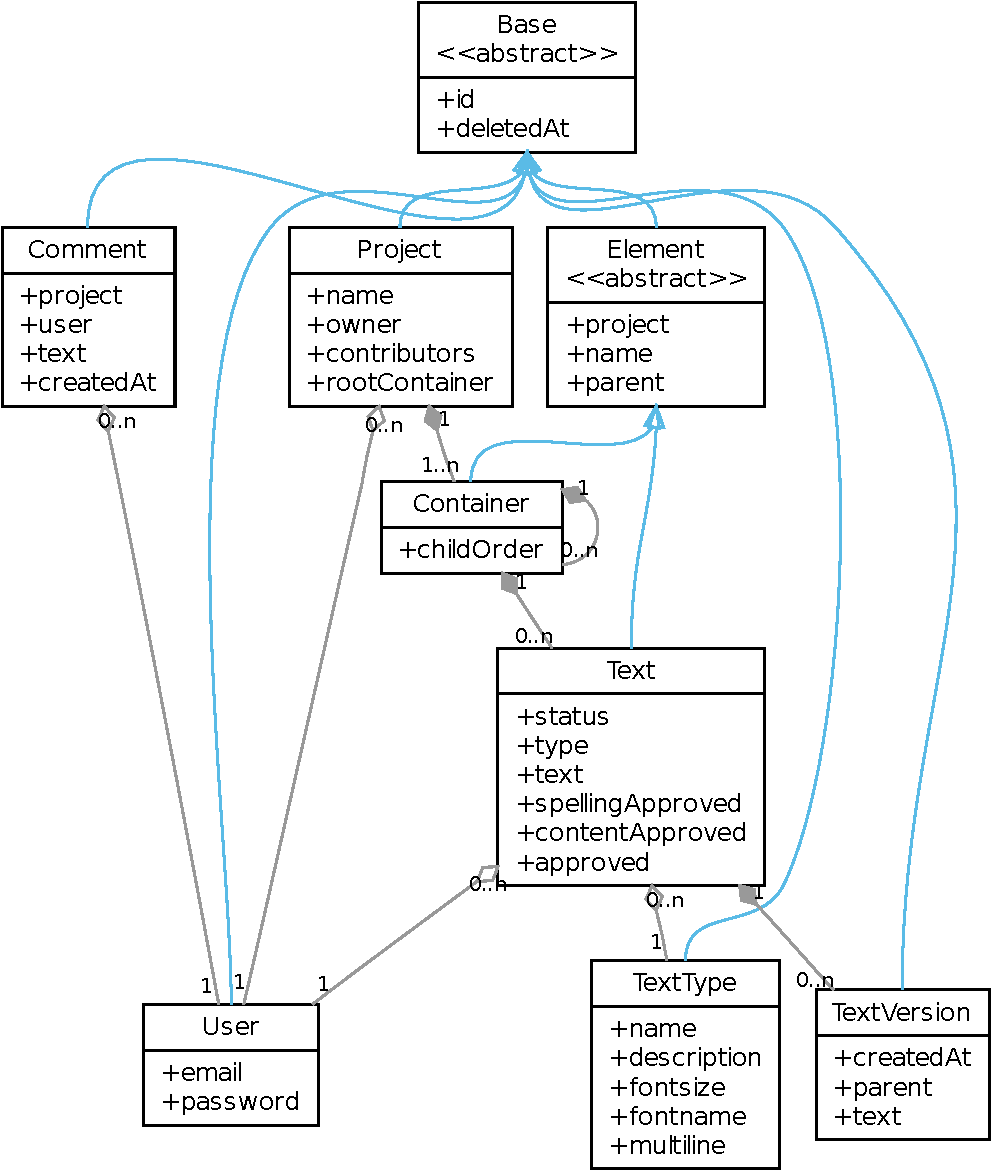
\includegraphics[width=0.65\textwidth]{media/prototyp-persistenz.pdf}
\captionof{figure}{Persistierte Objekte im Prototypen}\label{chart:prototype-persistenz}
\end{center}

Zum Persistieren der Daten kommt \trademark{MongoDB}\footnote{\url{http://www.mongodb.org/}}, eine No-SQL-Datenbank zum Einsatz, diese ermöglicht das unkomplizierte speichern auch komplexer Dokumentenstrukturen. Die Wahl einer nicht-relationen Datenbank bietet den Vorteil, dass aufwändiges Zusammensetzen und Zerlegen von Dokumenten entfallen kann. In der Datenbank werden die in Abbildung \ref{chart:prototype-persistenz} gezeigten Domänenobjekte gespeichert. Das Laden- und Speichern ist durch den Einsatz eines Object-Document-Mappers (ODM) für Doctrine 2 und MongoDB\footnote{\url{https://github.com/doctrine/mongodb-odm}} weitestgehend automatisiert. Dieses Modell ist deutlich einfacher als das in Abschnitt \ref{l:domänenmodell} / S.\pageref{l:domänenmodell} vorgestellte Domänenmodell, da im Prototyp nur wenige, entscheidende Funktionen implementiert wurden.

\subsubsection{Klassendiagramm}

\begin{center}
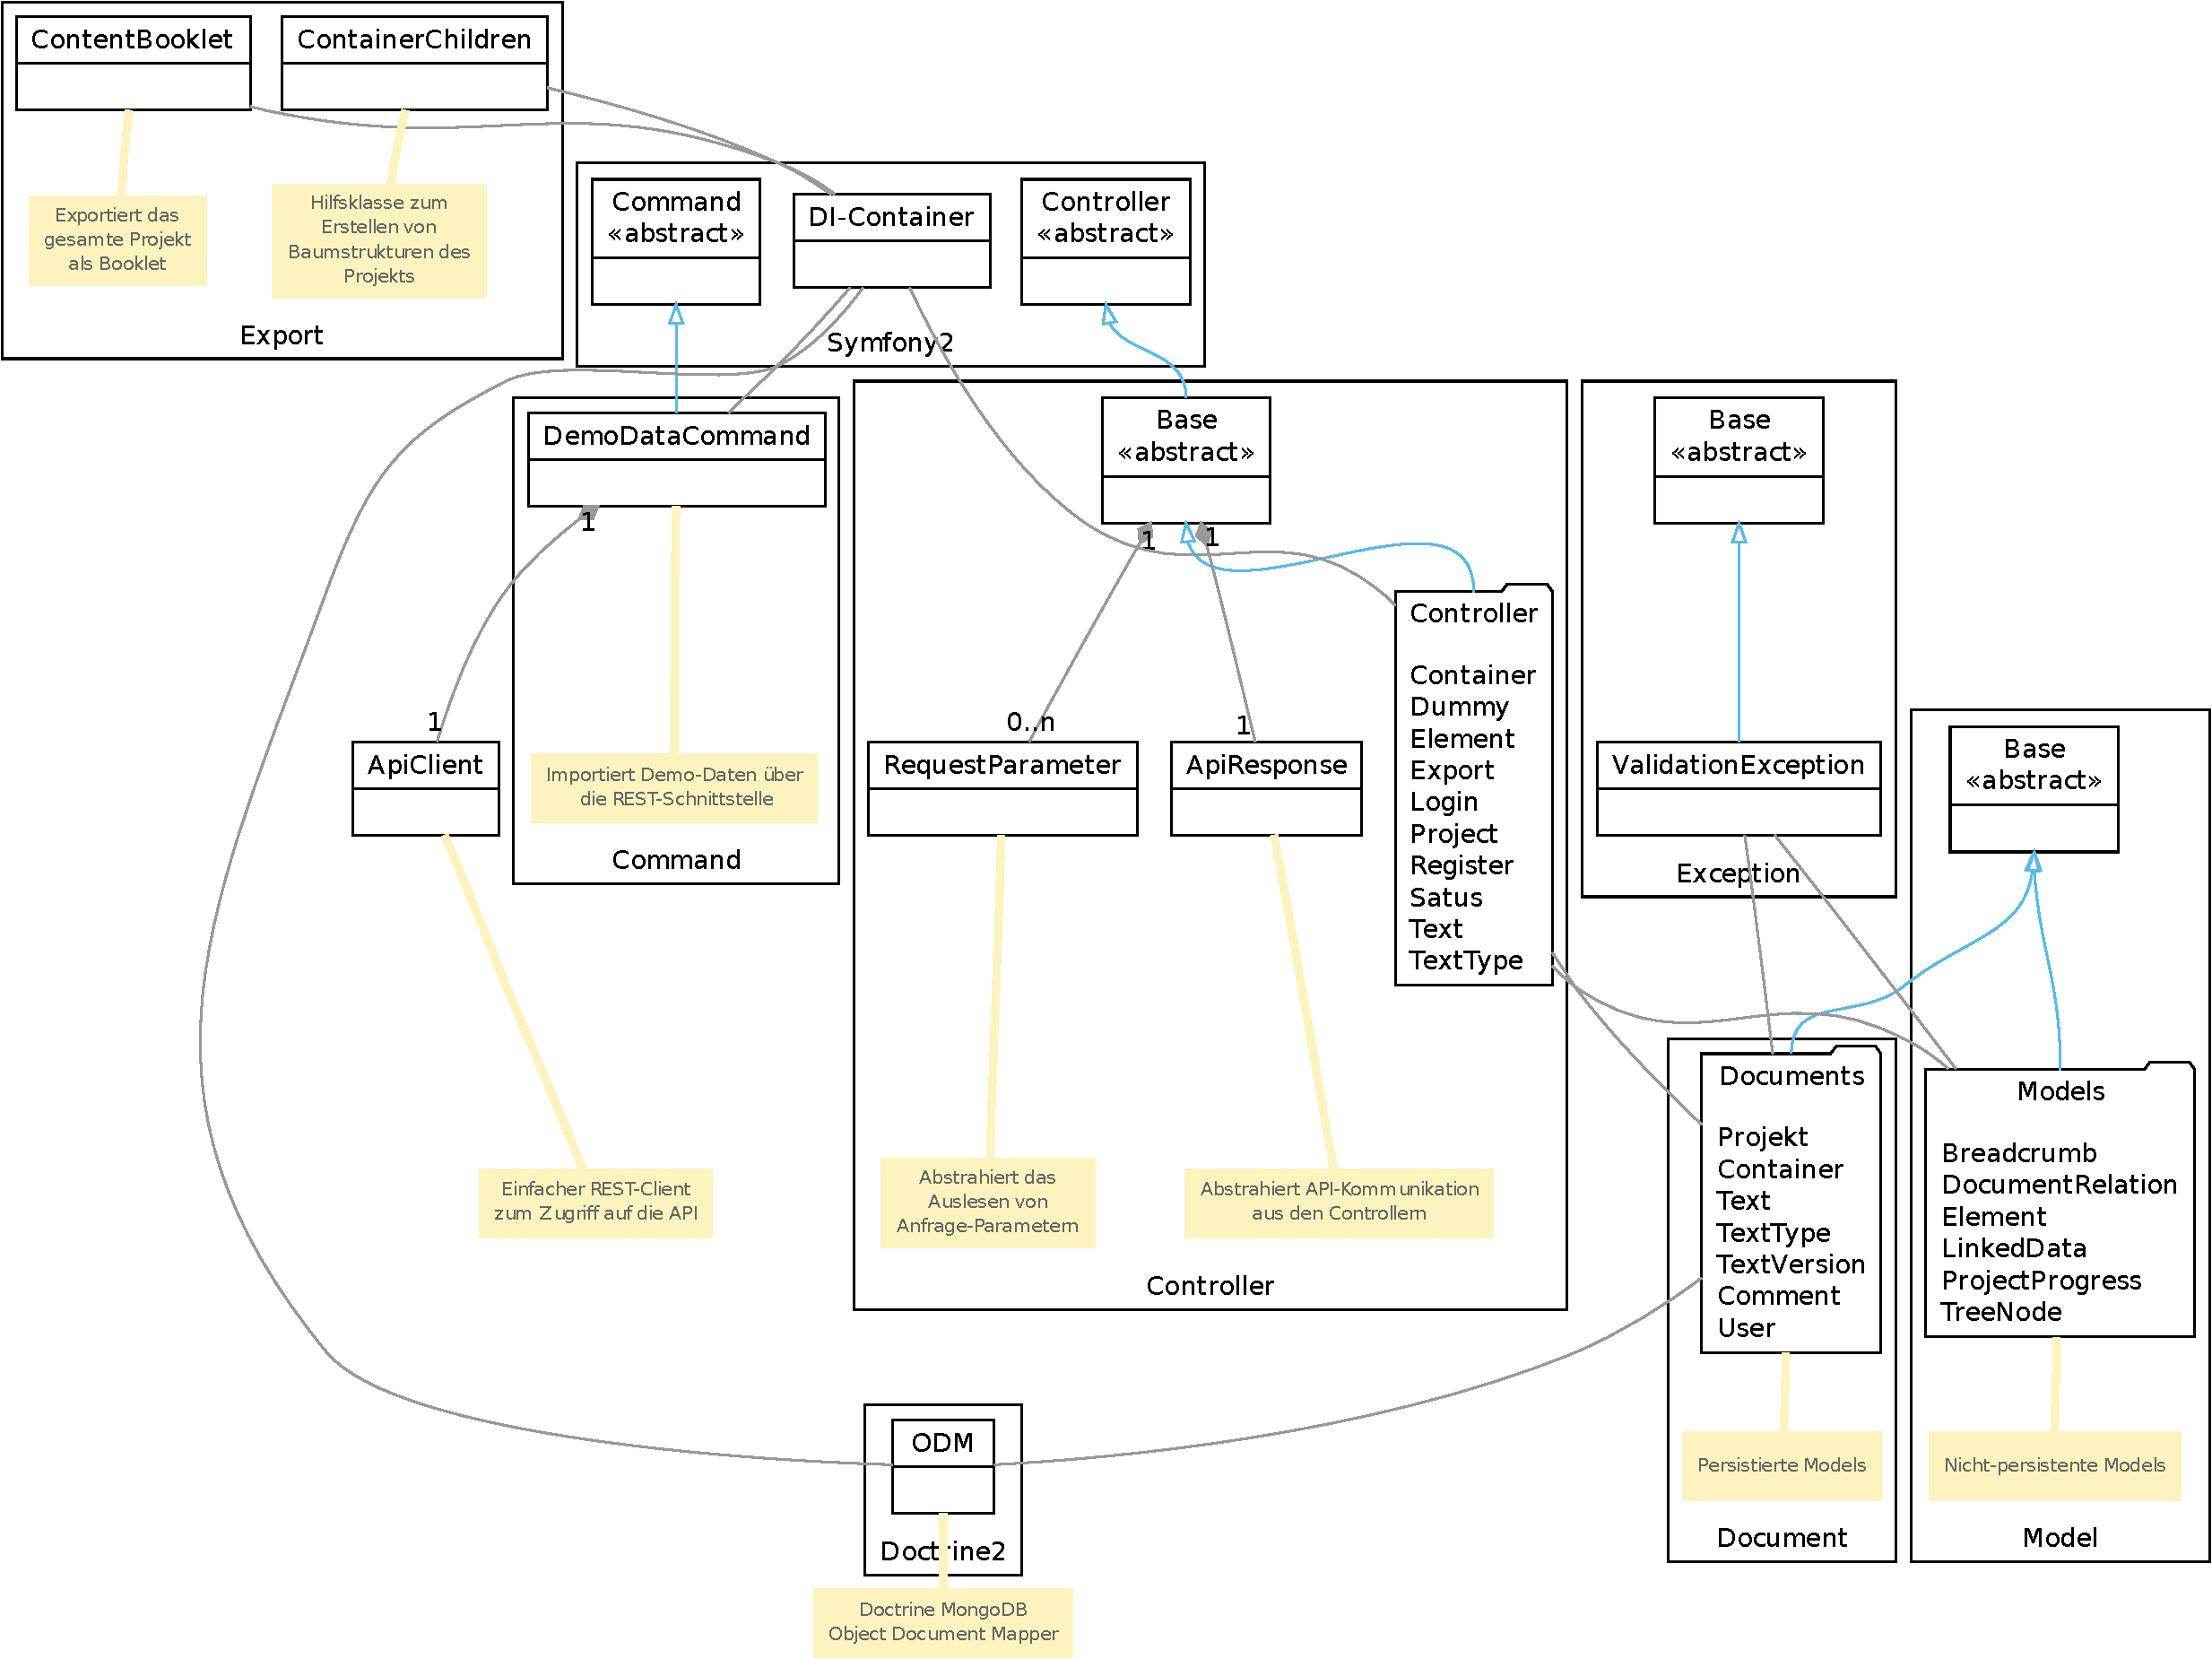
\includegraphics[width=\textwidth]{media/prototyp-klassendiagramm.pdf}
\captionof{figure}{Anwendungsserver-Klassendiagramm des Prototypen}\label{chart:prototyp-klassendiagramm}
\end{center}

Abbildung \ref{chart:prototyp-klassendiagramm} zeigt das Klassendiagramm der Implementierung des Prototypen. Zentrale Komponente ist der Dependency-Injection-Container (DI-Container) des Symfony2-Frameworks, dieser instanziert je nach Pfad der Anfrage einen Controller und ruft dort die entsprechende Methode auf. Dieses Listing zeigt die am Beispiel des \texttt{LoginControllers}, in dem die Methode \texttt{loginAction} aufgerufen wird, wenn der Pfad \texttt{\/login} lautet und die HTTP-Methode der Anfrage \texttt{POST} ist.

\begin{samepage}
\begin{verbatim}
class LoginController extends Base {
    /**
     * @Route("/login", requirements={"_method":"POST"})
     */
    public function loginAction() { … }
}
\end{verbatim}
\end{samepage}

Innerhalb der Controller steht der DI-Container zur Verfügung über den dann z.B. der ODM instanziert werden kann, um Daten aus der Datenbank zu laden. Der ODM verwendet zur Repräsentierung der Daten die Klassen aus dem Package \texttt{Documents}, die Controller können diese selber erzeugen, oder bekommen diese als Anfrage-Ergebnisse vom ODM übergeben.

Funktionen, die an mehreren Stellen, oder über unterschiedliche Arten verwendet werden, wurden in eigene Services ausgelagert (\texttt{ContentBooklet} und \texttt{ContainerChildren}). Diese werden zum einen innerhalb der Controller verwendet, können aber auch über das CLI gestartet werden. \trademark{Symfony2} stellt ein einfache Möglichkeit zum Erstellen vom Operationen über die Kommandozeile zur Verfügung. Im Prototyp wurde das Anlegen von Demo-Projekt-Daten mithilfe dieser Möglichkeit realisiert. Das \texttt{DemoDataCommand} wird von der Konsole aus gestartet und verwendet den \texttt{ApiClient}, um über HTTP mit der Schnittstelle des Anwendungsservers zu kommunizieren.
